% ==============================================================================
% SECCION 5: ACTIVIDAD 4 - REGLA DE MONOTONICIDAD, CASCADA DOMINO Y SKEW DE RELOJ
% ==============================================================================
\needspace{3\baselineskip}
\section{Actividad 4: Regla de Monotonicidad, Cascada Dominó y Skew de Reloj}
\label{sec:actividad4}

En la lógica CMOS dinámica, la salida solo puede realizar una transición descendente ($1 \to 0$) durante la fase de evaluación. Cuando múltiples compuertas dinámicas se interconectan directamente en cascada, el estado inicial pre-cargado ($1$ lógico) de la primera etapa puede activar transitoriamente la red de conmutación (PDN) de la etapa posterior antes de que la evaluación se complete, induciendo pérdidas de carga irreversibles. Esta sección analiza experimentalmente la violación de la regla de monotonicidad, valida su mitigación mediante la estructura dominó clásica (con inversor estático intermedio), examina la vulnerabilidad ante entradas no monótonas y contrasta el compromiso temporal y energético entre cascadas \textit{Footed} y \textit{Unfooted} frente al \textit{skew} de reloj.

\subsection{Violación de Monotonicidad y Prevención de Activación Prematura}
Se simuló una cascada de dos etapas dinámicas NAND2 idénticas ($W_n = 90\,\text{nm}, W_p = 135\,\text{nm}, W_{\text{PDN}} = 180\,\text{nm}$, $C_L = 2.0\,\text{fF}$) a $500\,\text{MHz}$ ($T_{clk} = 2.0\,\text{ns}$) bajo PTM 45\,nm HP. Se contrastaron tres regímenes operativos, documentados en la Figura~\ref{fig:monotonicidad_cascada}:

\begin{enumerate}[leftmargin=1.4em,itemsep=0.01em]
  \item \textbf{Régimen A (Cascada Directa Sin Inversor, $A=B=X=1$):} El nodo $dyn1$ conecta directo a la compuerta receptora. Al pasar a evaluación ($CLK: 0 \to 1$), $dyn1$ drena con retardo finito $t_{pHL1}$. Como $X=1$, la segunda etapa conduce a masa y vacía espuriamente a $dyn2$ hasta $V_{dyn2,\min} = \mathbf{0.64624\,\text{V}} \implies \Delta V_{dyn2} = \mathbf{353.76\,\text{mV}}$, erosionando el margen de ruido ($NM_H = 67.7\,\text{mV}$, pérdida del $84\%$), aunque sin bascular de inmediato ($V_{dyn2} > V_M \approx 0.48\,\text{V}$).
  \item \textbf{Régimen B (Cascada Dominó con Inversor, $A=B=X=1$):} Con inversor intermedio ($W_n = 90\,\text{nm}, W_p = 135\,\text{nm}$), $out1=0\,\text{V}$ en precarga. En evaluación, $out1$ ejecuta una transición \textbf{monótona creciente ($0 \to 1$)} solo tras evaluar la primera etapa, descargando legítimamente $dyn2$ a $\mathbf{-0.00584\,\text{V}} \approx 0\,\text{V}$ y evaluando la función lógica global ($out2 \approx 1.0\,\text{V}$).
  \item \textbf{Régimen C (Control de Bloqueo con Inversor, $A=B=1, X=0$):} Con $X=0$, la PDN2 permanece bloqueada pese a que $out1=1\,\text{V}$, reteniendo íntegramente $V_{dyn2,\min} = \mathbf{0.999999\,\text{V}}$ ($\Delta V \approx \mathbf{0.000\,\text{mV}}$, $out2 = 26.8\,\text{nV}$), confirmando el bloqueo funcional.
\end{enumerate}

\begin{figure}[htbp]
  \centering
  \begin{minipage}[t]{0.485\textwidth}
    \centering
    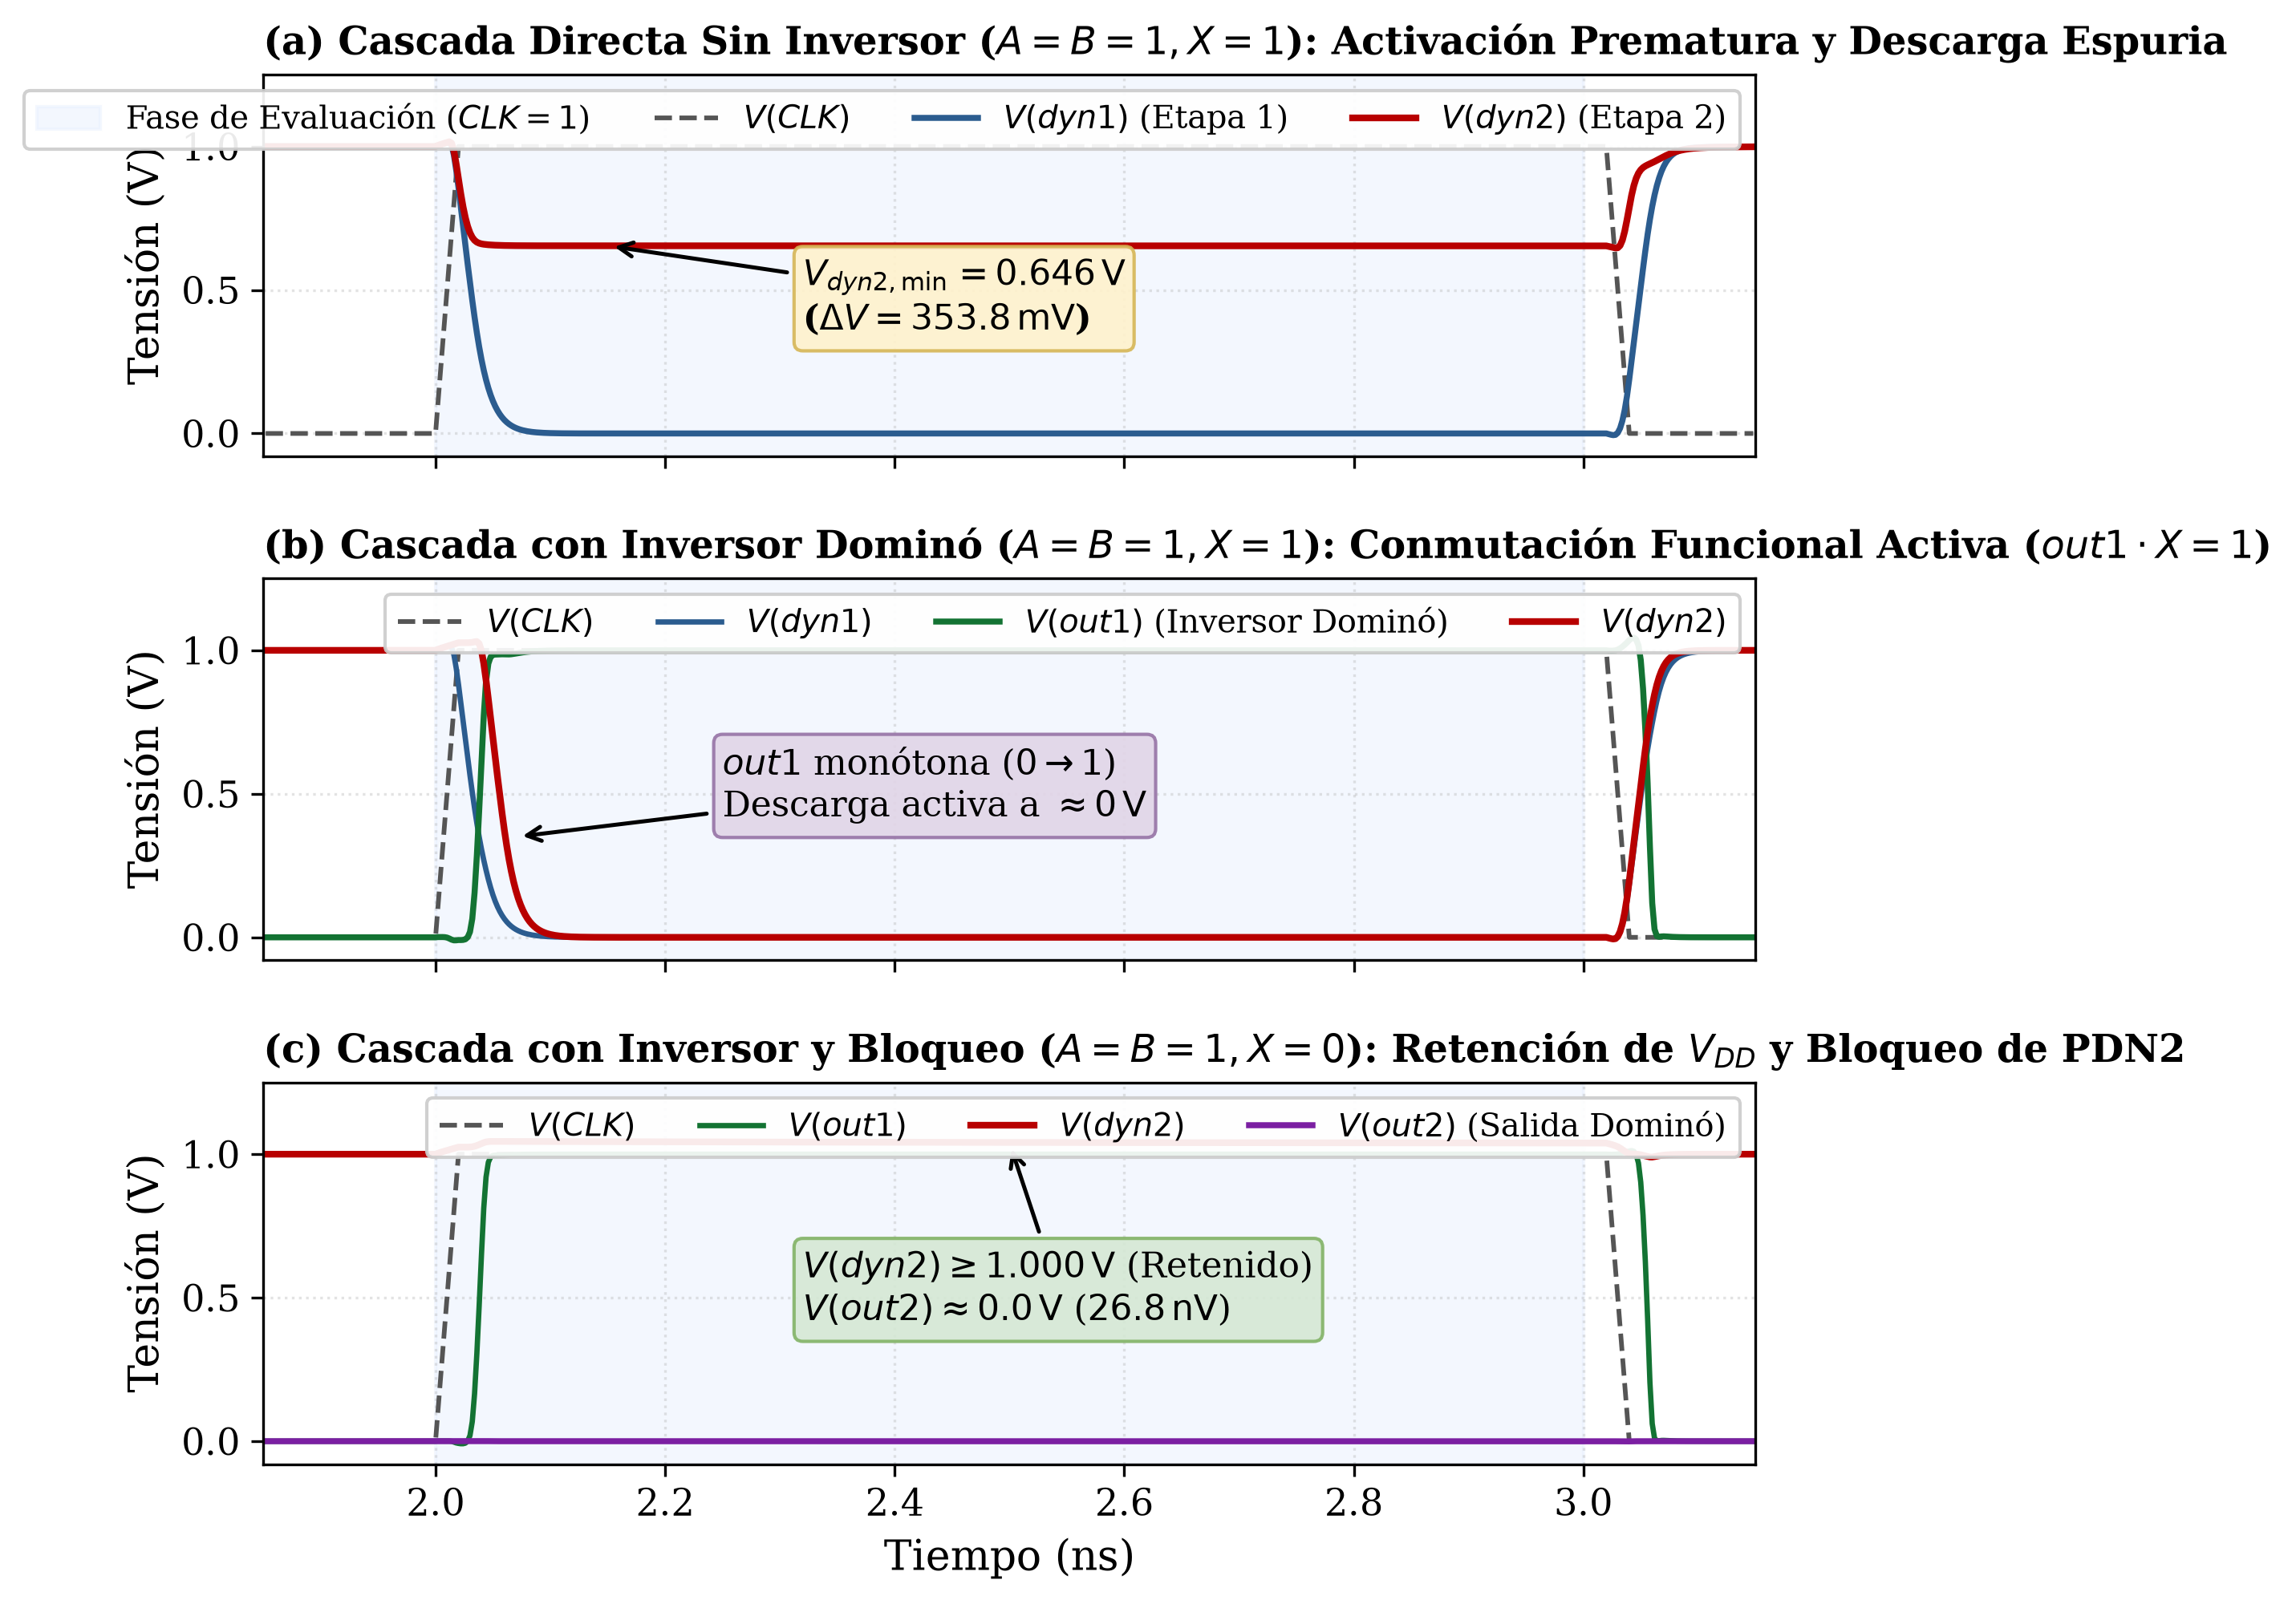
\includegraphics[width=\linewidth,height=4.3cm,keepaspectratio]{figuras/fig1_act4_monotonicidad_cascada.png}
    \caption[Análisis de regímenes de operación en cascada dominó]{Regímenes en cascada de 2 etapas NAND2 (45\,nm HP): (a) Directa sin inversor ($\Delta V = 353.8\,\text{mV}$); (b) Dominó ($dyn2 \approx 0\,\text{V}$); (c) Dominó con bloqueo ($X=0$, retención plena).}
    \label{fig:monotonicidad_cascada}
  \end{minipage}\hfill
  \begin{minipage}[t]{0.485\textwidth}
    \centering
    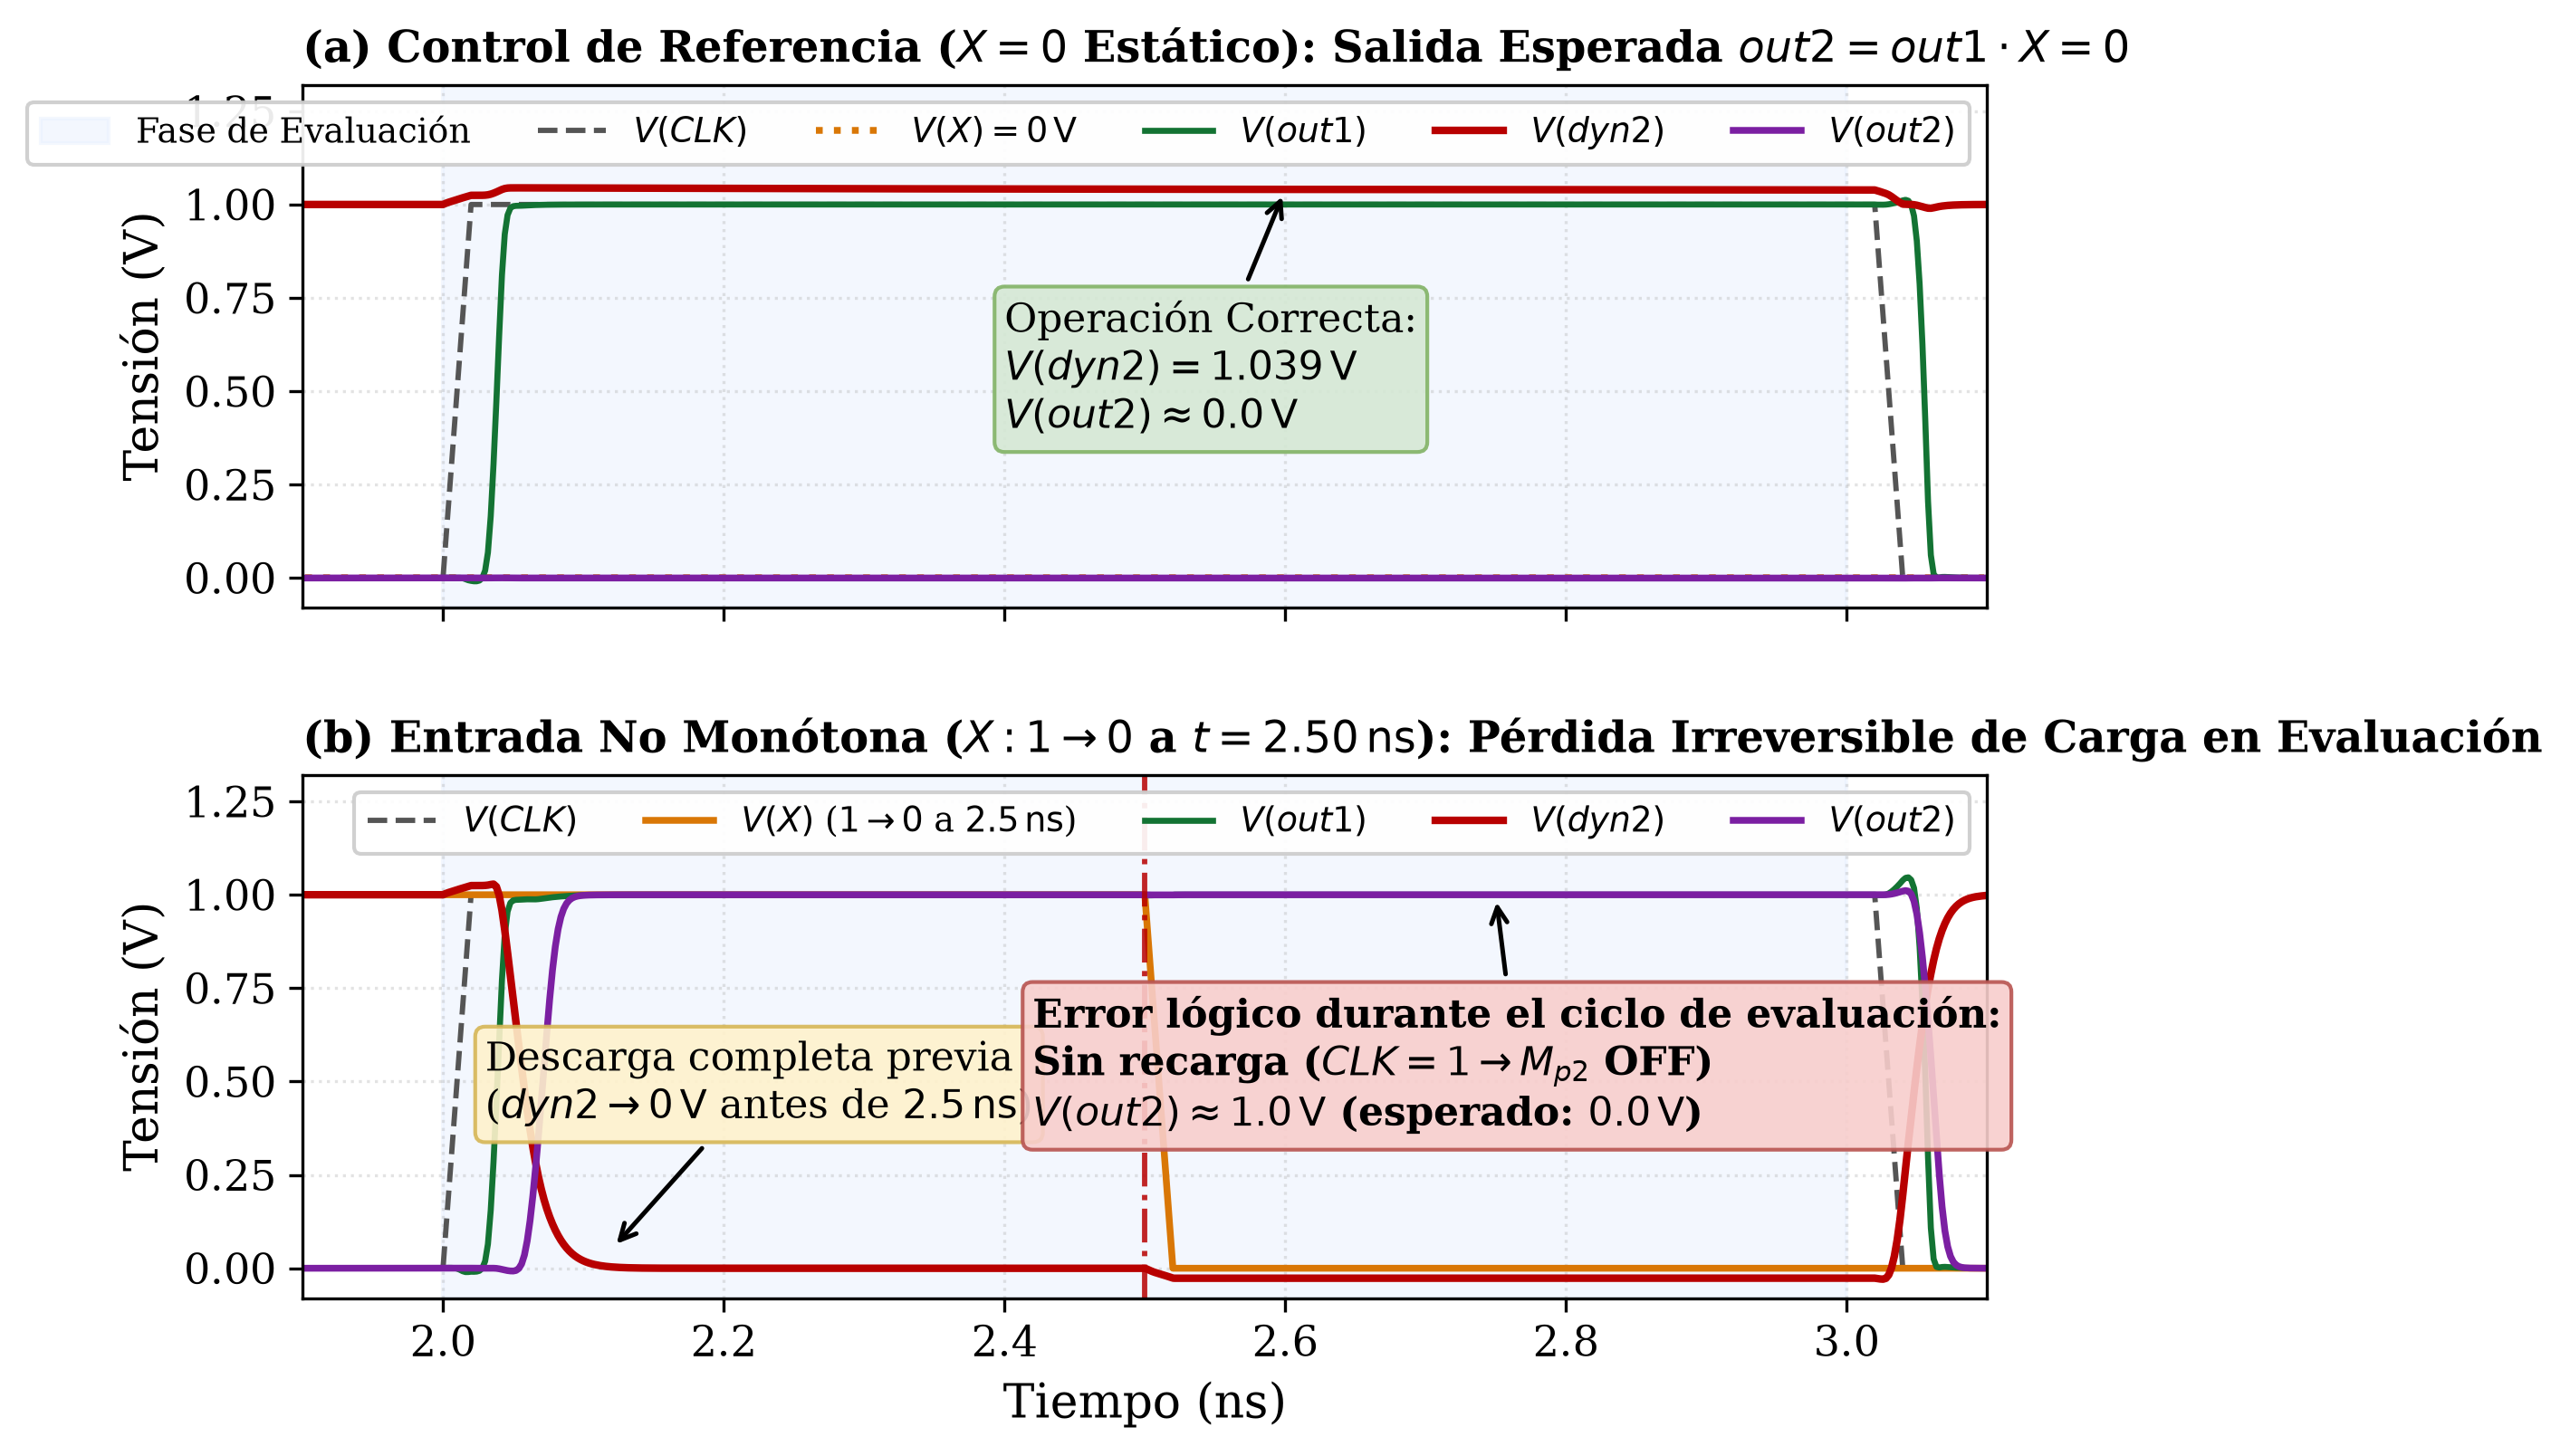
\includegraphics[width=\linewidth,height=4.3cm,keepaspectratio]{figuras/fig2_act4_pulso_x_descendente.png}
    \caption[Impacto de entrada externa no monótona]{Entrada externa no monótona (45\,nm HP): (a) Control $X=0$ estático ($out2 \approx 0\,\text{V}$); (b) Pulso descendente $X: 1 \to 0$ a $t=2.50\,\text{ns}$, evidenciando error lógico en ciclo activo.}
    \label{fig:pulso_x_descendente}
  \end{minipage}
\end{figure}

\subsection{Sensibilidad a Entradas Externas No Monótonas y Conexión con Flip-Flops}
Para evaluar la vulnerabilidad del nodo dinámico ante violaciones de la regla de monotonicidad en entradas externas, se modeló una compuerta dominó gobernada por $out1 \to 1$ donde la entrada externa $X$ experimenta una transición descendente ($1 \to 0$) a mitad de la fase de evaluación ($t = 2.50\,\text{ns}$). Los resultados se comparan con la referencia estática $X=0$:

\begin{itemize}[leftmargin=1.4em,itemsep=0.01em]
  \item \textbf{Descarga Previa a la Transición:} Entre $t=2.00\,\text{ns}$ y $t=2.50\,\text{ns}$, $X=1$ y $out1=1$. La PDN2 conduce y descarga $dyn2$ a tierra en $60\,\text{ps}$ ($V_{dyn2} = 3.66\,\mu\text{V}$ en $t=2.49\,\text{ns}$).
  \item \textbf{Interrupción sin Restauración:} A $t=2.50\,\text{ns}$, $X$ cae a $0\,\text{V}$ y apaga el NMOS inferior. Al estar el reloj en evaluación ($CLK=1$), el PMOS de precarga sigue cortado; al carecer de camino a $V_{DD}$, la carga \textbf{no se recupera en ese ciclo}.
  \item \textbf{Error Lógico en el Ciclo de Evaluación:} Al final de la fase ($t=2.99\,\text{ns}$), la lógica ideal exige $out2 = out1 \cdot X = 0$. Mientras el control estático entrega $out2 = 26.8\,\text{nV} \approx 0\,\text{V}$, con pulso se sostiene $dyn2 = -0.0265\,\text{V}$ y $out2 = \mathbf{0.999997\,\text{V}} \approx 1.0\,\text{V}$, constituyendo un \textbf{error lógico funcional por vaciado irreversible}.
  \item \textbf{Implicancia para Biestables (TGFF):} Las señales excitadoras desde biestables deben asegurar transiciones monótonas crecientes o niveles estables sin \textit{glitches} durante la evaluación para evitar la corrupción de datos.
\end{itemize}

\subsection{Cascada Dominó de Tres Etapas: Footed vs Unfooted y Skew de Reloj}
Para cuantificar el impacto del desalineamiento de reloj en cascadas de mayor profundidad lógica, se evaluó una estructura dominó NAND2 de 3 etapas en versiones \textit{Footed} (con $M_f$) y \textit{Unfooted} (sin $M_f$) bajo un barrido de skew temporal ($T_{\text{skew}} \in [-50, 200]\,\text{ps}$). La Tabla~\ref{tab:skew_act4} y la Figura~\ref{fig:footed_vs_unfooted_skew} consolidan las mediciones.

% Tabla de caracterizacion de cascada domino de 3 etapas Footed vs Unfooted bajo barrido de skew de reloj
% Fuente primaria: Tarea 4 Footed.log y Paso 5 Unfooted.log (PTM 45nm HP, VDD = 1.0 V, T = 27 C)
\begin{table}[htbp]
\centering
\fontsize{7.5pt}{8.8pt}\selectfont
\caption[Caracterización de cascada dominó de 3 etapas Footed vs Unfooted]{Respuesta temporal y picos de corriente de alimentación en cascada dominó de 3 etapas (NAND2) bajo barrido de skew de reloj ($T_{\text{skew}} \in [-50, 200]\,\text{ps}$): contraste entre arquitecturas Footed y Unfooted.}
\label{tab:skew_act4}
\begin{tabularx}{\linewidth}{@{}>{\centering\arraybackslash}p{1.2cm} c c c c c c >{\RaggedRight\arraybackslash}X@{}}
\toprule
\textbf{$T_{\text{skew}}$} & \textbf{$t_{\text{del}}$ (Foot)} & \textbf{$t_{\text{del}}$ (Unfoot)} & \textbf{$\Delta t_{\text{del}}$} & \textbf{$I_{\text{pk}}$ (Foot)} & \textbf{$I_{\text{pk}}$ (Unfoot)} & \textbf{$\Delta I_{\text{pk}}$} & \textbf{Diagnóstico Físico / Condición de Operación} \\
\textbf{(ps)} & \textbf{(ps)} & \textbf{(ps)} & \textbf{(\%)} & \textbf{($\mu\text{A}$)} & \textbf{($\mu\text{A}$)} & \textbf{($\mu\text{A}$)} & \textbf{(Ventana de medición: $t \in [0.5, 4.5]\,\text{ns}$)} \\
\midrule
$-50$ & 77.20 & 66.46 & $-13.9\%$ & 113.80 & 326.30 & $+212.50$ & Precarga adelantada en etapas 2 y 3 drena a través de la PDN en conducción. \\
$0$   & 77.21 & 66.47 & $-13.9\%$ & 318.85 & 332.91 & $+14.06$  & Sincronismo pleno: las 3 etapas precargan simultáneamente en paralelo. \\
$+50$ & 125.47 & 95.12 & $-24.2\%$ & 110.56 & 110.57 & $+0.01$   & Desacoplo de precargas; corriente limitada al pico capacitivo de una etapa. \\
$+100$& 226.68 & 130.81& $-42.3\%$ & 110.56 & 160.57 & $+50.01$  & Incremento de corriente en unfooted por conducción simultánea PMOS/PDN. \\
$+200$& 426.91 & 171.48& $-59.8\%$ & 110.56 & 214.63 & $+104.07$ & Elevación de pico de alimentación ($+94.1\%$); Footed inmune a corto. \\
\bottomrule
\end{tabularx}
\end{table}


\begin{itemize}[leftmargin=1.4em,itemsep=0.0em]
  \item \textbf{Ahorro a Skew Nulo ($T_{\text{skew}}=0\,\text{ps}$):} \textit{Unfooted} reduce el retardo de $77.21\,\text{ps}$ a $66.47\,\text{ps}$ ($\Delta t = \mathbf{-10.74\,\text{ps}}$, ahorro del $\mathbf{-13.9\%}$) al suprimir transistores $M_f$.
  \item \textbf{Sensibilidad a Skew Positivo ($T_{\text{skew}} > 0$):} A $+200\,\text{ps}$, \textit{Footed} retrasa a $426.91\,\text{ps}$ sin sobrecorriente. \textit{Unfooted} propaga en $171.48\,\text{ps}$ pero dispara la corriente a $214.63\,\mu\text{A}$ ($\Delta I_{\text{pk}} = \mathbf{+104.07\,\mu\text{A}}$, $+94.1\%$) por conducción solapada PMOS/PDN.
  \item \textbf{Skew Negativo ($T_{\text{skew}}=-50\,\text{ps}$):} El adelanto de reloj dispara la corriente en \textit{Unfooted} a $I_{\text{pk}} = 326.30\,\mu\text{A}$ vs $113.80\,\mu\text{A}$ en \textit{Footed}, confirmando que el desfasaje negativo es crítico.
  \item \textbf{Criterio de Rabaey:} Suprimir el footer exige que el corte de la etapa previa preceda a la conducción receptora; la lógica unfooted exige un estricto control temporal bidireccional para no disparar corriente.
  \item \textbf{Difusión Parásita:} Incluir $AS/AD/PS/PD$ incrementa el retardo global de $77.21\,\text{ps}$ a $89.90\,\text{ps}$ ($+16.43\%$) con corriente casi invariable ($-1.9\%$).
\end{itemize}

\begin{figure}[htbp]
  \centering
  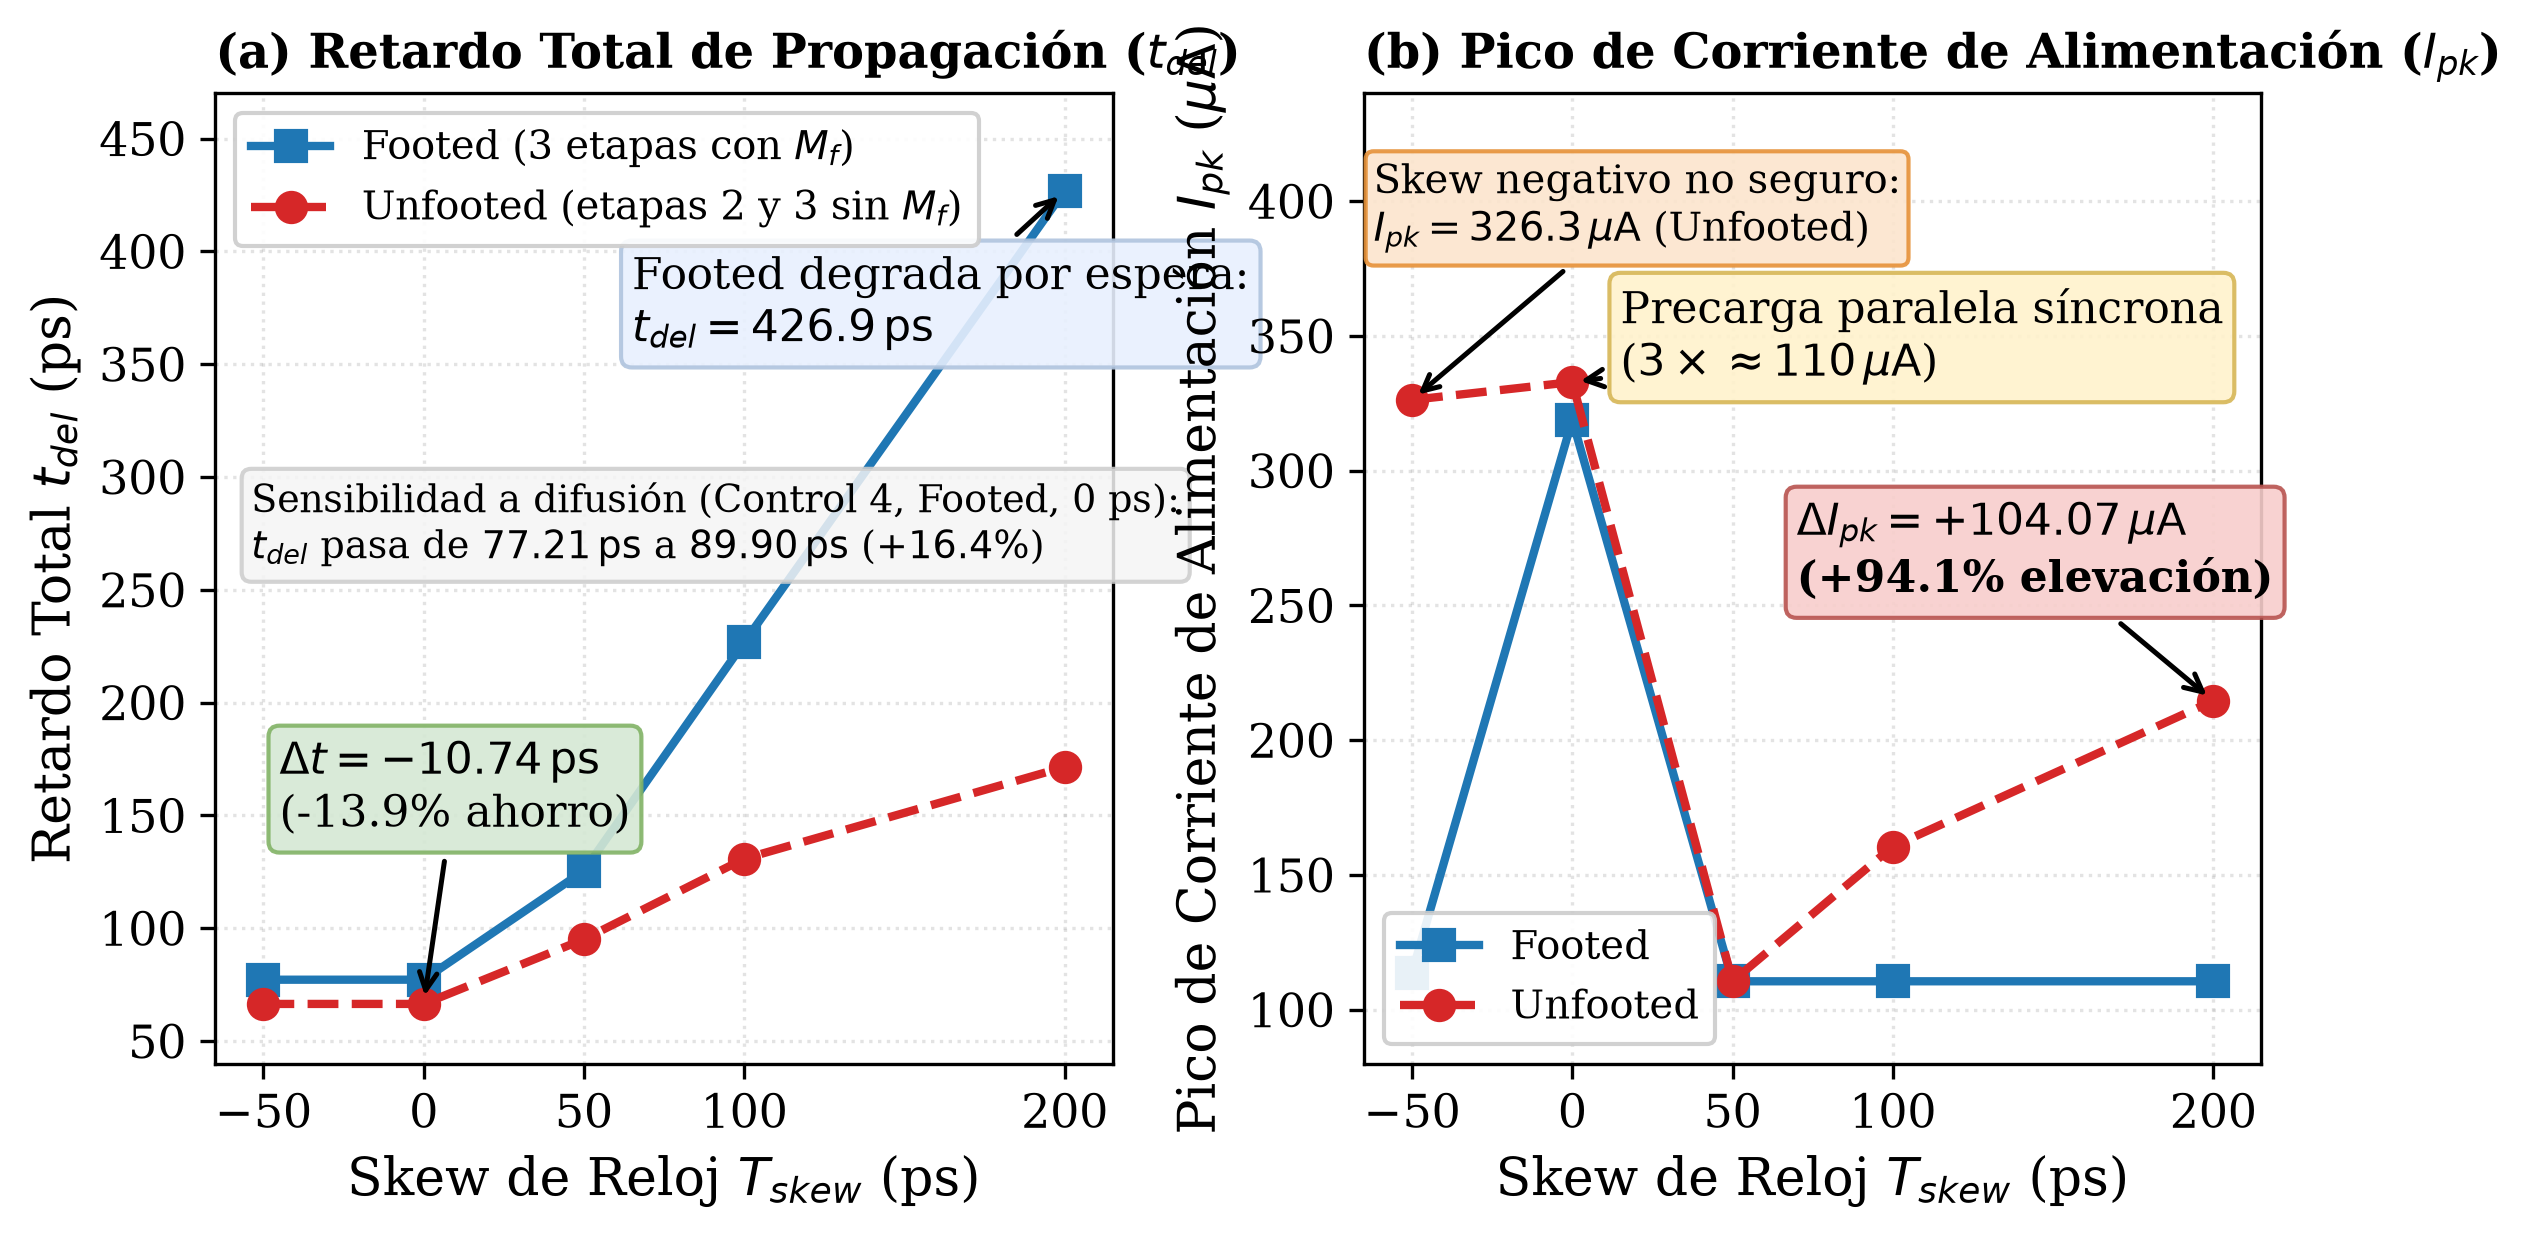
\includegraphics[width=0.55\linewidth,height=2.7cm,keepaspectratio]{figuras/fig3_act4_footed_vs_unfooted_skew.png}
  \caption[Sensibilidad al skew de reloj en cascada dominó de 3 etapas]{Sensibilidad al skew de reloj en cascada dominó de 3 etapas (PTM 45\,nm HP): (a) Retardo total de propagación $t_{\text{del}}$ vs $T_{\text{skew}}$; (b) Pico de corriente de alimentación $I_{\text{pk}}$ vs $T_{\text{skew}}$.}
  \label{fig:footed_vs_unfooted_skew}
\end{figure}

\subsection{Conclusiones de la Actividad 4}
\begin{enumerate}[leftmargin=1.4em,itemsep=0.0em]
  \item \textbf{Eficacia del Inversor Dominó:} La cascada directa sin inversor sufre una descarga espuria de $353.76\,\text{mV}$ ($\Delta NM_H = -84\%$) por activación prematura de la PDN. El inversor estático asegura transiciones monótonas crecientes ($0 \to 1$), garantizando retención íntegra de $V_{DD}$ ante $X=0$ y conmutación activa funcional cuando $X=1$.
  \item \textbf{Monotonicidad en Entradas Externas:} La caída de una entrada externa ($X: 1 \to 0$) produce un error lógico en dicho ciclo ($out2 \approx 1.0\,\text{V}$ en vez de $0\,\text{V}$) porque la descarga precede a la transición y la carga no se repone con $CLK=1$. Esto exige que los biestables excitadores (ej. TGFF) sean rigurosamente monótonos y sin glitches.
  \item \textbf{Compromiso Footed vs Unfooted:} Prescindir del footer ahorra $13.9\%$ de retardo a skew nulo, pero a $T_{\text{skew}}=+200\,\text{ps}$ eleva el pico de alimentación en $+104.07\,\mu\text{A}$ ($+94.1\%$) y a $-50\,\text{ps}$ genera $326.30\,\mu\text{A}$. La celda Footed brinda inmunidad robusta frente a desalineamientos temporales.
\end{enumerate}
